% Slide 35
\begin{frame}{Model-based Policy Optimization}
\vspace{1em}
How to augment?
\begin{itemize}
    \item Generate full trajectories from initial states?
\end{itemize}
\end{frame}

% Slide 36
\begin{frame}{Model-based Policy Optimization}
\vspace{1em}
How to augment?
\begin{itemize}
    \item Generate full trajectories from initial states?
    \begin{itemize}
        \item Model may not be accurate for long horizons
    \end{itemize}
\end{itemize}
\end{frame}

% Slide 37
\begin{frame}{Model-based Policy Optimization}
\vspace{1em}
How to augment?
\begin{itemize}
    \item Generate full trajectories from initial states?
    \begin{itemize}
        \item Model may not be accurate for long horizons
    \end{itemize}
    \item Generate partial trajectories from initial states?
\end{itemize}
\end{frame}

% Slide 38
\begin{frame}{Model-based Policy Optimization}
\vspace{1em}
How to augment?
\begin{itemize}
    \item Generate full trajectories from initial states?
    \begin{itemize}
        \item Model may not be accurate for long horizons
    \end{itemize}
    \item Generate partial trajectories from initial states?
    \begin{itemize}
        \item May not get good coverage of later states
    \end{itemize}
\end{itemize}
\end{frame}

% Slide 39
\begin{frame}{Model-based Policy Optimization}
\vspace{1em}
How to augment?
\begin{itemize}
    \item Generate full trajectories from initial states?
    \begin{itemize}
        \item Model may not be accurate for long horizons
    \end{itemize}
    \item Generate partial trajectories from initial states?
    \begin{itemize}
        \item May not get good coverage of later states
    \end{itemize}
    \item Generate partial trajectories from all states in the data
\end{itemize}
\end{frame}

% Slide 40: same content + the real-vs-augmented trajectory diagram
\begin{frame}{Model-based Policy Optimization}
\begin{columns}[c]
\begin{column}{0.56\textwidth}
\vspace{1em}
How to augment?
\begin{itemize}
    \item Generate full trajectories from initial states?
    \begin{itemize}
        \item Model may not be accurate for long horizons
    \end{itemize}
    \item Generate partial trajectories from initial states?
    \begin{itemize}
        \item May not get good coverage of later states
    \end{itemize}
    \item Generate partial trajectories from all states in the data
\end{itemize}
\end{column}
\begin{column}{0.44\textwidth}
\centering
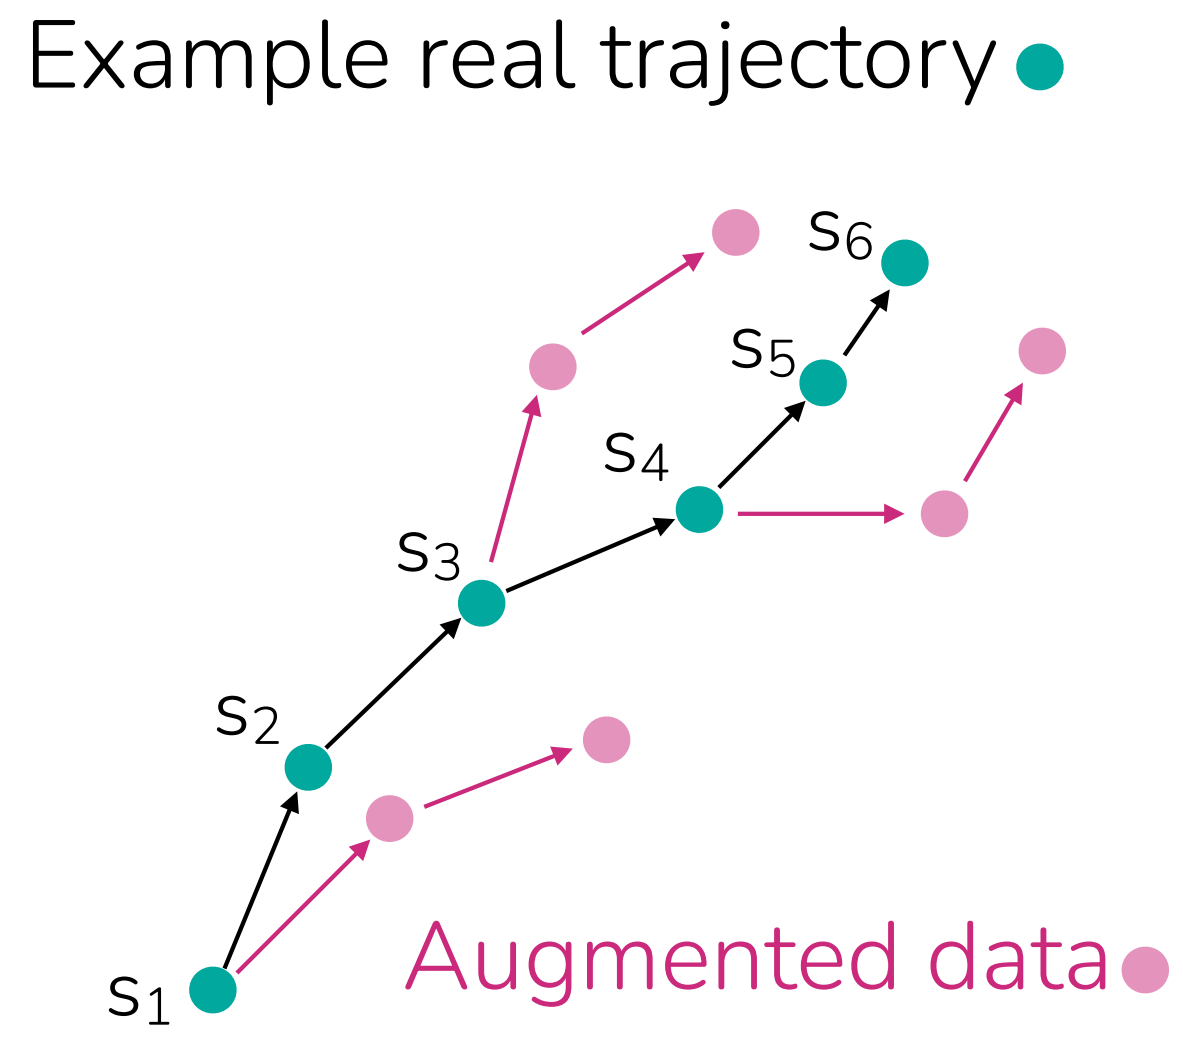
\includegraphics[width=\linewidth,height=0.78\textheight,keepaspectratio]{images/model-based-rl/figures/augment-trajectory.jpg}
\end{column}
\end{columns}
\end{frame}
